\documentclass[11pt]{article}

\usepackage[margin=1in]{geometry}
\usepackage{amsmath}
\usepackage{amssymb}
\usepackage{booktabs}
\usepackage{graphicx}
\graphicspath{{figures/}}
\usepackage{microtype}
\usepackage{xcolor}
\usepackage[colorlinks=true,linkcolor=blue,citecolor=blue,urlcolor=blue]{hyperref}

% --- lightweight macros ---
\newcommand{\dphi}{d_{\phi}}
\newcommand{\dhd}{d_{h}}
\newcommand{\R}{\mathbb{R}}
\newcommand{\quadtwo}{\textsc{quad2}}

\title{\textbf{Prizma-Seq: A Parameter-Free Quadratic\\ Delta-State Sequence Mixer}}
\author{Aylin\\ \small Independent Researcher}
\date{}

\begin{document}
\maketitle

\begin{abstract}
We present \emph{Prizma-Seq}, a Gated-DeltaNet--family sequence mixer whose only added lever is
a \emph{parameter-free quadratic feature map} (\quadtwo) that lifts each head's keys and queries
from dimension $\dhd{=}32$ to $\dphi{=}256$ using fixed seeded monomial buffers. Because the
monomial coefficients are seeded constants rather than learned weights, \quadtwo{} adds
\emph{zero} parameters while making the per-head carried associative state \emph{rectangular}
($\dhd\times\dphi$ rather than $\dhd\times\dhd$), which preserves exact $O(1)$-per-step,
constant-memory inference. Parameter-matched against a tuned decoder-only Transformer
(RMSNorm + SwiGLU + RoPE), Prizma-Seq clears a pre-registered, falsifiable diagnostic bar at small
scale: it reaches descriptive parity on MQAR ($D{=}128$) at $\sim$860K matched parameters, solves
$D{=}128$ at 130K parameters where the matched Transformer fails and the smallest Transformer
solver on our coarse grid needs $\geq$461K ($\geq$3.5$\times$ parameter-efficiency); it solves
induction (0.9995) and selective-copy (0.9991); and it is competitive on a text8 character LM
(1.7496 vs.\ 1.7254 bits-per-character, within a pre-registered $+0.05$ margin --- it does
\emph{not} beat the Transformer). At inference the carried state is a constant $0.56$\,MB ($147{,}456$ fp32 floats) at every
sequence length --- analytically $28$--$455\times$ fewer floats than a growing KV-cache --- which
shows up as a measured constant $17.9$\,MB peak (weights $+$ activations $+$ state) versus the
Transformer's $49.5$--$561.7$\,MB, i.e.\ a $2.8$--$31\times$ measured peak-memory advantage; and a
measured $O(1)$-latency crossover appears at $n{\geq}32\text{k}$ ($2.4$--$2.8\times$ faster at
$n{=}65\text{k}$); below $\sim$16k it is $\sim$1.3--1.6$\times$ \emph{slower}. A causal ablation shows the gain is the quadratic
monomials specifically ($\quadtwo\!\gg\!\text{rand\_linear}\!\approx\!\text{none}\!\gg\!\text{TF}$),
not ``a bigger recurrent state.'' We make no per-FLOP, large-scale-LM, or backprop-free-parity
claim; Prizma-Seq is a \emph{candidate} efficient-attention replacement in the tested regime, and
the \quadtwo{} kernel itself belongs to the Based/Hedgehog feature-map family --- the contribution
here is the \emph{rectangular delta-state} framing.
\end{abstract}

\section{Introduction}
\label{sec:intro}

Self-attention~\cite{vaswani2017attention}'s score matrix costs $O(n^2)$ compute and an $O(n)$
growing KV-cache at decode time, which dominates the cost of long-context generation. A now-large family of \emph{efficient
attention replacements} --- linear attention~\cite{katharopoulos2020transformers}, state-space
models~\cite{gu2022s4,gu2024mamba}, and delta-rule recurrences~\cite{yang2024deltanet,
yang2024gateddeltanet} --- replace the score matrix with a carried associative state of fixed size,
trading the $O(n^2)$ matrix for $O(n\cdot\dhd^2)$ training and, crucially, $O(\dhd^2)$
\emph{per-step, sequence-length-independent} inference. The practical promise is constant-memory,
constant-latency decoding at long context.

The cost of this trade is \emph{recall}: a fixed-rank state can store fewer associations than an
unbounded KV-cache, and this shows up directly on associative-recall diagnostics such as
MQAR~\cite{arora2024zoology}. The Based and Hedgehog lines~\cite{arora2024based,zhang2024hedgehog}
recover much of this recall by passing keys and queries through an expressive (often quadratic)
\emph{feature map} before forming the state, enlarging the effective key space.

This paper studies a single, deliberately narrow question: \emph{can a parameter-free quadratic
feature map, used to make a Gated-DeltaNet state rectangular, match a tuned Transformer on the
field-standard attention-diagnostic suite at matched parameters while preserving $O(1)$
inference?} Our answer, scoped to small scale and the named tasks, is yes. We call the resulting
mixer \emph{Prizma-Seq}. Its lever, \quadtwo, lifts each head's keys/queries from $\dhd{=}32$ to
$\dphi{=}256$ using \emph{fixed seeded monomial buffers}: the lift is a function with no learnable
parameters, so it adds zero to the parameter budget, and it turns the per-head state from a square
$\dhd\times\dhd$ matrix into a \emph{rectangular} $\dhd\times\dphi$ matrix. Because the state size is
still independent of $n$, the constant-memory / $O(1)$-per-step inference property is preserved
exactly.

We test Prizma-Seq against a pre-registered, falsifiable bar (Section~\ref{sec:setup}) and report
every number with its honest caveat (Section~\ref{sec:limits}). We emphasize up front what is
\emph{not} claimed: Prizma-Seq does not beat the Transformer on the character LM (it is within a
margin), the latency advantage is long-context-only, the architecture is $\sim$5$\times$ slower to
train per step, we make no per-FLOP claim, and we make no large-scale-LM or backprop-free-parity
claim. The contribution is the \textbf{rectangular delta-state framing} of a known kernel, not a
new kernel.

\section{Method}
\label{sec:method}

\subsection{The Gated-DeltaNet backbone}
Prizma-Seq replaces self-attention's token mixer; everything else --- the SwiGLU
FFN~\cite{shazeer2020glu}, RMSNorm~\cite{zhang2019rmsnorm}, RoPE~\cite{su2021roformer} on the
encoder projections, token embeddings, and the tied output head, in the
Llama-family style~\cite{touvron2023llama} --- is byte-identical to our Transformer baseline, so
\emph{only the mixer differs}. This makes the comparison a clean attention-replacement test rather
than a whole-architecture confound.

Within each head, the mixer carries an associative state $S_t$ updated by a precision-gated
\emph{delta rule}~\cite{yang2024deltanet,schlag2021linear} with a data-dependent forget gate
$\alpha_t$~\cite{yang2024gateddeltanet,gu2024mamba}:
\begin{equation}
S_t \;=\; \alpha_t\, S_{t-1} \;+\; \beta_t\,\varepsilon_t\, k_t^{\top},
\qquad
\varepsilon_t \;=\; v_t - S_{t-1} k_t,
\label{eq:delta}
\end{equation}
where $k_t$ are $L_2$-normalized keys, $v_t$ values, $\beta_t=\sigma(W_\beta x_t)$ an
input-dependent write gate, and $\varepsilon_t$ the prediction error (the ``surprise'') of the
current value under the running state. Reads are recognition-by-reconstruction
$o_t = S_{t-1} q_t$, augmented by a small exact local-window head ($w{=}16$) of the kind used in
Based/Griffin~\cite{arora2024based,de2024griffin}. A short causal depthwise convolution (kernel 4),
standard in Mamba/Based/DeltaNet, precedes the projections.

Equation~\eqref{eq:delta} is exactly one gradient step on a per-token \emph{free energy}
$F_t(S)=\tfrac12\lVert v_t - S k_t\rVert^2$, since
$\partial F_t/\partial S = -(v_t - S k_t)k_t^{\top} = -\varepsilon_t k_t^{\top}$. This
predictive-coding reading~\cite{rao1999predictive,friston2010free} of the delta write is the
project's framing of the mechanism; the components themselves are borrowed and known-good, and we
disclose this explicitly (Section~\ref{sec:related}). The distinct, separately-tested lever is the
feature map below.

\subsection{The \quadtwo{} parameter-free quadratic feature map}
The Based/Hedgehog insight~\cite{arora2024based,zhang2024hedgehog} is that passing keys/queries
through a quadratic feature map $\phi(\cdot)$ before forming the state recovers much of the recall
that a linear state loses. We adopt this kernel family but in a specific, parameter-free form.
For a head dimension $\dhd{=}32$, define $\phi:\R^{\dhd}\!\to\!\R^{\dphi}$ with $\dphi{=}256$ by
\emph{fixed seeded monomials}: the linear terms $u_i$ plus a fixed, seeded selection of
second-order cross-products $u_i u_j$,
\begin{equation}
\phi(u) \;=\; \big[\, u_1,\dots,u_{\dhd},\;\; u_{a_1}u_{b_1},\, u_{a_2}u_{b_2},\,\dots,\,
u_{a_m}u_{b_m} \,\big] \in \R^{\dphi},
\label{eq:quad2}
\end{equation}
where the index pairs $\{(a_r,b_r)\}_{r=1}^{m}$ are drawn \emph{once} from a fixed seed and stored
as constant integer buffers (here $m=224$ cross-terms plus the $32$ linear terms give
$\dphi{=}256$). Crucially, $\phi$ has \emph{no learnable parameters}: the monomial structure is a
seeded constant, so \quadtwo{} adds \textbf{zero parameters} to the model. Parameter-matching to the
Transformer is therefore exact-by-construction --- the projection budget is unchanged.

\subsection{Rectangular delta-state and why $O(1)$ inference survives}
Replacing the keys $k_t$ in Equation~\eqref{eq:delta} with their lifted form $\phi(k_t)\in\R^{\dphi}$
(and reading with $\phi(q_t)$) turns the carried state from a square $\dhd\times\dhd$ matrix into a
\textbf{rectangular} $\dhd\times\dphi$ matrix:
\begin{equation}
S_t \;=\; \alpha_t\, S_{t-1} \;+\; \beta_t\,\varepsilon^{\phi}_t\,\phi(k_t)^{\top},
\qquad
\varepsilon^{\phi}_t \;=\; v_t - S_{t-1}\,\phi(k_t),
\qquad S_t \in \R^{\dhd\times\dphi},
\qquad o_t \;=\; S_{t-1}\,\phi(q_t).
\label{eq:rectstate}
\end{equation}
This is the paper's contribution: the \emph{rectangular delta-state framing}
(Fig.~\ref{fig:arch}). The predictive-coding reading carries over with the lifted key: the write
$\beta_t\varepsilon^{\phi}_t\phi(k_t)^{\top}$ is one gradient step on
$F_t(S)=\tfrac12\lVert v_t - S\,\phi(k_t)\rVert^2$, whose gradient is
$\partial F_t/\partial S = -\varepsilon^{\phi}_t\phi(k_t)^{\top}$. The recall ceiling is
governed by the effective rank of the lifted key space ($\dphi$ near-orthogonal directions per head
rather than $\dhd$), recovering associative capacity, while the per-token write and read remain a
pair of matrix-vector products over a state of \emph{fixed} size $\dhd\dphi$ floats. Because that
size does not depend on the sequence length $n$, the inference profile is unchanged from the linear
case: per-step cost is $O(\dhd\dphi)$ and the carried state is constant in $n$. We verified that the
single-step recurrence and the chunk-parallel training form agree
($\lVert\text{step}-\text{forward}\rVert<10^{-6}$: none $3.6\times10^{-7}$, \quadtwo{}
$4.8\times10^{-7}$), so the cheap inference path is the exact same model as the trained one.

\begin{figure}[t]\centering
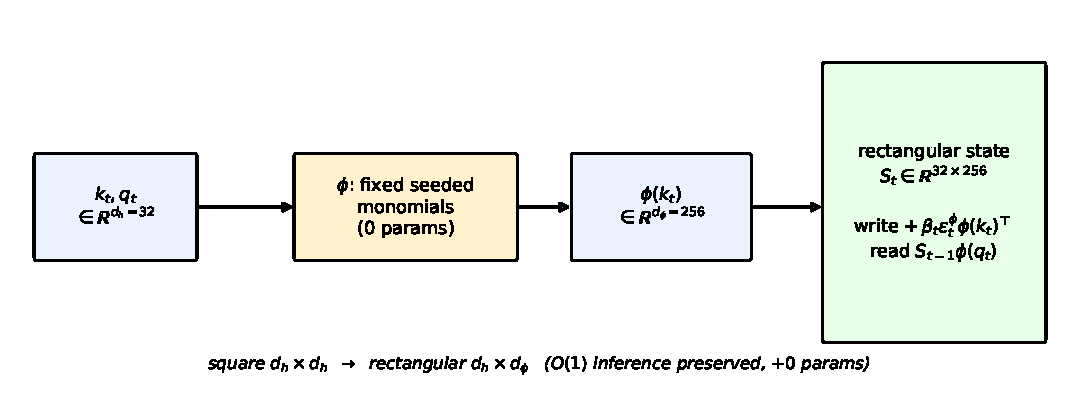
\includegraphics[width=0.92\linewidth]{fig1_architecture.pdf}
\caption{The \quadtwo{} lift makes the per-head delta-state \emph{rectangular}
($\dhd\times\dphi$) at zero added parameters; the per-token write and read stay matrix--vector
products over a state whose size $\dhd\dphi$ is independent of the sequence length $n$, so $O(1)$
inference is preserved.}
\label{fig:arch}
\end{figure}

The cost of the lift is FLOPs, not parameters or memory: the $\dphi{=}256$ expansion multiplies the
delta-state FLOPs and brings Prizma-Seq's forward cost to $2.14\times$ (as-coded; $1.78\times$
kernel-ideal) the Transformer's per token at the headline scale (Section~\ref{sec:limits}). We make no per-FLOP claim and disclose this ratio
plainly.

\section{Experimental setup}
\label{sec:setup}

\paragraph{Pre-registered falsifiable bar.}
Before running the headline experiments we committed to a falsifiable bar consisting of the
field-standard attention diagnostics plus a structural-advantage and a causal-attribution leg. The
pass conditions (e.g.\ MQAR parity within noise at matched parameters; induction $\geq$0.98 with the
64--256 gap bin $\geq$0.95; selective-copy $\geq$0.97 with a fixed-position control; character LM
test BPC $\leq T+0.05$; constant-memory inference; and a causal control in which a random
\emph{linear} map matches the no-feature-map baseline) were fixed in advance. A leg can fail; the
report states whatever the experiment shows.

\paragraph{Baseline and parameter-match auditor.}
The baseline is a tuned decoder-only Transformer with RMSNorm, SwiGLU, and RoPE, sharing the FFN,
norms, embeddings, and tied head with Prizma-Seq so that only the mixer differs. A parameter-match
auditor counts both models at each scale; the headline MQAR scale d128L4H4 is matched to
\textbf{TF 857{,}216 vs.\ Prizma-quad2 862{,}368 params ($+0.6\%$)}, and the character-LM scale to
TF 3{,}220{,}480 vs.\ Prizma-quad2 3{,}224{,}608 ($+0.13\%$). Scale notation is
$d\{$model$\}$L$\{$layers$\}$H$\{$heads$\}$; throughout, $\dhd{=}32$ and \quadtwo{} uses $\dphi{=}256$.

\paragraph{Protocol and honesty notes.}
MQAR and induction exhibit a seed-dependent phase transition at this scale \emph{for both}
architectures, so we report median, solve-rate ($>$0.9), and seed range over $\geq$3 seeds rather
than a fragile mean. The MQAR/induction/selective-copy/causal legs ran at a single shared
$\text{lr}{=}10^{-3}$ (the Transformer's tuned value, which is \emph{conservative for} Prizma-Seq,
disadvantaging it, not the baseline); only the character LM swept a per-model learning rate. We
disclose two reproducibility caveats binding on the diagnostic legs: per-seed weight init is not
bit-pinned by the seed in those runs (the comparison is symmetric across architectures, but
absolute solve-rates are not bit-reproducible), and the seed counts ($n{=}3$ diagnostics,
$n{=}2$ character LM) are \emph{descriptive}, not powered equivalence tests. Inference \emph{memory}
is analytically counted from closed-form float counts; inference \emph{latency} is measured
wall-clock on an A100 (median of 5 reps, 2 warmup). All experiments are small scale on the named
tasks --- exactly what the bar pre-registered.

\section{Results}
\label{sec:results}

Table~\ref{tab:bar} reports the seven legs of the pre-registered bar with headline numbers. All four
field-standard diagnostic legs (MQAR, induction, selective-copy, character LM) pass parameter-matched
against the tuned Transformer; the structural-advantage leg passes on memory at every length and on
latency only at long context; the causal leg attributes the gain to the quadratic monomials; and
length extrapolation is a \emph{relative} win.

\begin{table}[t]
\centering
\small
\caption{Prizma-Seq against the pre-registered, parameter-matched bar (tuned Transformer baseline,
A100). Numbers are medians over seeds; see Sections~\ref{sec:infer}--\ref{sec:limits} for caveats.
Char-LM is reported as competitive \emph{within} the $+0.05$ margin, \emph{not} a win.}
\label{tab:bar}
\begin{tabular}{@{}llp{8.2cm}@{}}
\toprule
\textbf{Leg} & \textbf{Verdict} & \textbf{Headline} \\
\midrule
MQAR ($D{=}128$) & PASS &
Parity at 860K matched params (\quadtwo{} median 0.998 vs.\ TF 0.9995); solves at 130K where the
matched TF fails (0/3) and the smallest grid TF solver needs $\geq$461K $\Rightarrow$
$\geq$3.5$\times$ param-efficiency (coarse grid). \\
\addlinespace[2pt]
Induction & PASS &
\quadtwo{} median 0.9995 (3/3) vs.\ TF 0.9956. \emph{Non-discriminating:} Prizma-none also solves
(1.0). \\
\addlinespace[2pt]
Selective-copy & PASS &
Selective median 0.9991 ($\geq T{-}0.02$); fixed-position control isolates content-selectivity
(spread $10^{-4}$). \emph{Non-discriminating:} Prizma-none also solves. \\
\addlinespace[2pt]
Char-LM (text8) & PASS &
Prizma 1.7496 vs.\ TF 1.7254 BPC; margin $-0.024 < +0.05$. Within the bar; does \textbf{not} beat
the TF. \\
\addlinespace[2pt]
Inference & PASS (memory) &
Constant $0.56$\,MB analytic state ($28$--$455\times$ fewer floats than KV); measured constant
$17.9$\,MB peak ($2.8$--$31\times$ less than TF); $O(1)$-latency crossover at $n{\geq}32$k
($2.4$--$2.8\times$ faster at $n{=}65$k). \\
\addlinespace[2pt]
Causal ablation & PASS &
$\quadtwo$ (3/3, 0.997) $\gg$ rand\_linear ($\approx$0.59) $\approx$ none ($\approx$0.52) $\gg$ TF
(0.016). The gain is the monomials, not ``a bigger RNN.'' \\
\addlinespace[2pt]
Length-extrapolation & WIN (relative) &
Retention at $8\times$ train length: Prizma 0.398 vs.\ RoPE-TF 0.041 ($\sim$10$\times$). Absolute
acc still only $\sim$0.40 at $8\times$. \\
\bottomrule
\end{tabular}
\end{table}

\paragraph{MQAR: parity and parameter-efficiency.}
At $\sim$860K matched parameters (d128L4H4, 3 seeds), all three arms solve $D{=}128$: Prizma-quad2
seeds $[0.9991, 0.9983, 0.9955]$ (median 0.9983) vs.\ Transformer $[0.9787, 0.9995, 0.9998]$
(median 0.9995). With $n{=}3$ at ceiling we cannot resolve a difference --- this is descriptive
parity (a failure-to-reject), not a tested equivalence. At matched params Prizma-quad2 (0.9983) also
exceeds Prizma-none (median 0.9583), and ignites fastest of the three (by step 16--20k, vs.\ TF
44--80k). At the smaller 130K scale (d64L2H2), Prizma-quad2 solves $D{=}128$ (3/3, seeds
$[0.999, 0.997, 0.935]$, median 0.997) where the param-matched Transformer fails (0/3, 0.016). The
smallest Transformer that solves $D{=}128$ on our coarse 4-point grid $\{130, 461, 857, 3300\}$K is
d128L2H4 (461K), giving a $\geq$3.5$\times$ parameter-efficiency gap (Fig.~\ref{fig:mqar}). We flag that one quad2 seed
(0.935) is borderline (clearing the 0.9 bar by 0.035) and that a denser Transformer sweep (200--450K)
is needed to pin the true crossover.

\begin{figure}[t]\centering
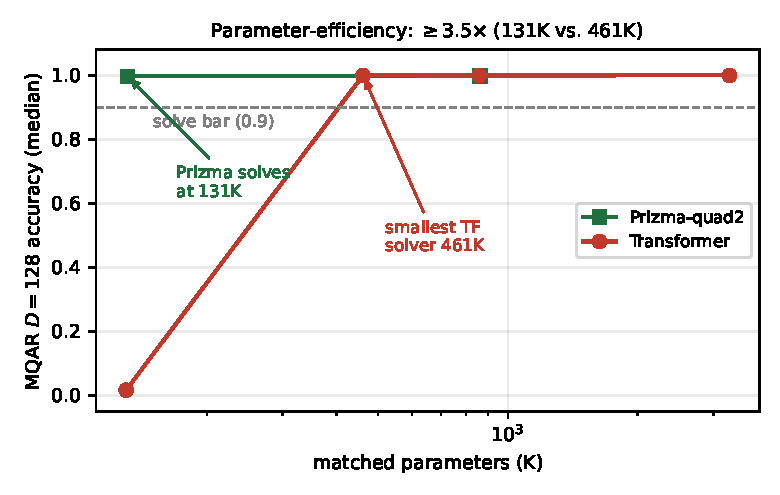
\includegraphics[width=0.7\linewidth]{fig4_mqar.pdf}
\caption{MQAR ($D{=}128$) median accuracy vs.\ matched parameters (3 seeds; 5 for the 857K TF).
Prizma-quad2 solves at 131K where the param-matched Transformer fails ($0.016$); the smallest
Transformer solver on the coarse grid $\{130,461,857,3300\}$K is d128L2H4 at 461K, giving a
$\geq$3.5$\times$ parameter-efficiency gap. All points trace to \texttt{results/gpu\_bench.json}.}
\label{fig:mqar}
\end{figure}

\paragraph{Capacity question, resolved honestly.}
A sufficiently large Transformer \emph{does} solve $D{=}128$ (d128L2H4/461K: 3/3, 0.9999;
d256L4H8/3.3M: 3/3). The tiny-Transformer failure is under-capacity at that size, not ``attention
cannot recall.'' The honest differentiators are parameter-efficiency and $O(1)$-memory inference ---
never ``attention fails.''

\paragraph{Induction and selective-copy.}
Both pass parameter-matched (d128L2H4, $0.64\%$ match): induction \quadtwo{} median 0.9995 (3/3,
0.9995 at the 256-gap bin) vs.\ TF 0.9956; selective-copy \quadtwo{} median 0.9991 vs.\ TF 0.9994,
with the fixed-position control spread at $10^{-4}$. We disclose that these two legs are
\emph{non-discriminating}: Prizma-none also solves them, so the feature-map's edge is visible in the
MQAR-param-efficiency and causal-ablation legs, not here.

\paragraph{Character LM (text8).}
On text8~\cite{mahoney2011text8} (train 10M / val 0.5M / test 0.5M chars, $V{=}27$,
AdamW~\cite{loshchilov2019adamw,kingma2015adam} $\text{wd}{=}0.1$, val-based early stopping,
$n{=}2$ seeds), Prizma-quad2 reaches median test 1.7496 BPC vs.\ Transformer 1.7254 BPC ---
a margin of $-0.024$, within the pre-registered $+0.05$ bar and far below the random baseline of
4.7549. We state plainly: Prizma-Seq is competitive \emph{within} the margin and does \textbf{not}
beat the Transformer here. Neither arm overfits (final BPCs 1.76 / 1.74). The Prizma arm took
$\sim$1889\,s vs.\ the Transformer's $\sim$361\,s ($\sim$5.2$\times$ slower to train).

\section{Inference efficiency}
\label{sec:infer}

The structural advantage of a fixed-size carried state is constant inference memory. Decoding via
\texttt{model.step()} (KV-cache for the Transformer, $O(1)$ state for Prizma-Seq) on an A100, the
\emph{analytic} carried state is $\dhd\dphi$ floats per head; at the small config it totals
$147{,}456$ fp32 floats $=0.56$\,MB, \emph{constant in $n$}, against a KV-cache that grows from
$4{,}194{,}304$ floats ($n{=}4$k) to $67{,}108{,}864$ ($n{=}65$k) --- an analytic $28.4\times$ to
$455\times$ float advantage. This shows up as a \emph{measured} peak process memory (model weights
$+$ activations $+$ state) that is a \textbf{constant 17.9\,MB} for Prizma-Seq at every length,
while the Transformer's measured peak grows from 49.5\,MB ($n{=}4$k) to 561.7\,MB ($n{=}65$k) --- a
measured peak advantage of $2.8\times$ to $31.4\times$. The larger config shows the same pattern
(Prizma 232\,MB constant vs.\ TF 491\,MB $\to$ 4532\,MB).

\begin{figure}[t]\centering
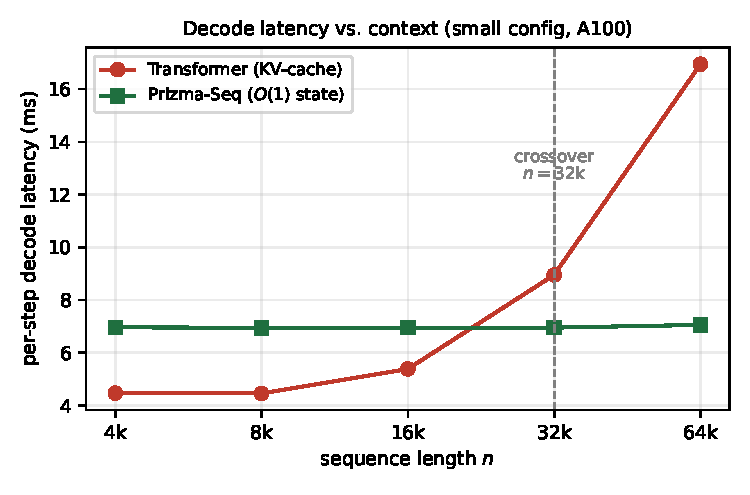
\includegraphics[width=0.62\linewidth]{fig2_latency.pdf}\\[3pt]
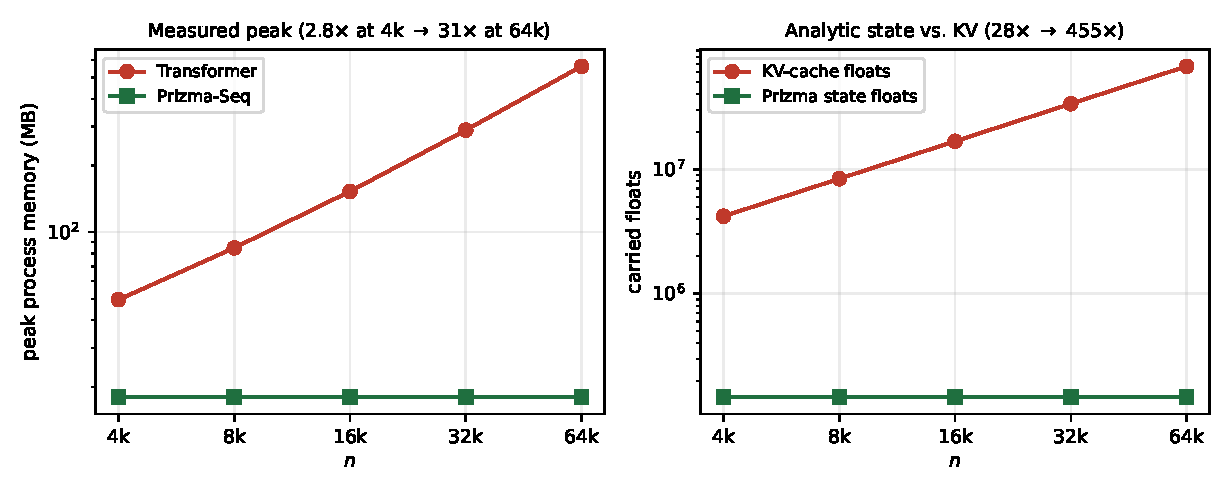
\includegraphics[width=0.95\linewidth]{fig3_memory.pdf}
\caption{Inference profile (A100, small config). Top: per-step decode latency is flat for
Prizma-Seq and crosses the Transformer at $n{=}32$k. Bottom: the carried state is constant in $n$ ---
$28$--$455\times$ fewer floats than the KV-cache (right, analytic) and $2.8$--$31\times$ less
measured peak memory (left). Data: \texttt{results/gpu\_latency.json}.}
\label{fig:infer}
\end{figure}

\begin{table}[t]
\centering
\small
\caption{Measured per-step decode latency (ms) and peak memory (MB) vs.\ sequence length $n$ on an
A100 (small config: d128L4H4, $\dhd{=}32$, $\dphi{=}256$). Prizma-Seq latency is flat ($O(1)$); the
Transformer grows. The latency crossover is at $n{=}32$k; below $\sim$16k Prizma-Seq is slower
(overhead-bound). Peak mem is measured process peak (weights $+$ activations $+$ state), not the
$0.56$\,MB analytic state.}
\label{tab:latency}
\begin{tabular}{@{}lrrrrr@{}}
\toprule
$n$ & 4{,}096 & 8{,}192 & 16{,}384 & 32{,}768 & 65{,}536 \\
\midrule
TF latency (ms)        & 4.47 & 4.46 & 5.39 & 8.95 & 16.95 \\
Prizma latency (ms)    & 6.96 & 6.95 & 6.95 & 6.95 & 7.06 \\
\addlinespace[2pt]
TF peak mem (MB)       & 49.5 & 84.9 & 152.8 & 289.1 & 561.7 \\
Prizma peak mem (MB)   & 17.9 & 17.9 & 17.9 & 17.9 & 17.9 \\
\bottomrule
\end{tabular}
\end{table}

Table~\ref{tab:latency} and Figure~\ref{fig:infer} report measured per-step latency. Prizma-Seq's latency is statistically flat
across a $16\times$ span of $n$ ($\sim$7\,ms throughout), while the Transformer grows from 4.47\,ms to
16.95\,ms. The wall-clock \emph{latency} crossover is at $n{=}32{,}768$; at $n{=}65$k Prizma-Seq is
$2.4\times$ faster (small config: 7.06 vs.\ 16.95\,ms) and $2.8\times$ faster on the larger config
(13.87 vs.\ 38.90\,ms). \textbf{Below $n\lesssim$16k Prizma-Seq is $\sim$1.3--1.6$\times$ slower}
(it is overhead-bound at short context): the latency win is long-context-only and we disclose it as
such. The memory advantage, by contrast, holds at every length.

\section{Ablation: is it the quadratic monomials?}
\label{sec:ablation}

To rule out the alternative explanation that the gain is merely ``a bigger recurrent state'' (a wider
$\dphi$), we run a causal control (Fig.~\ref{fig:ablation}) at d64L2H2 (130K) on MQAR $D{=}128$ with three feature-map
conditions plus the Transformer, all at fixed $\text{lr}{=}2\times10^{-3}$ (3 seeds):
\begin{equation*}
\underbrace{\quadtwo}_{\text{3/3, med }0.997} \;\gg\;
\underbrace{\text{rand\_linear}}_{\text{0/3, med }0.589} \;\approx\;
\underbrace{\text{none}}_{\text{0/3, med }0.518} \;\gg\;
\underbrace{\text{TF}}_{\text{0/3, }0.016}.
\end{equation*}

\begin{figure}[t]\centering
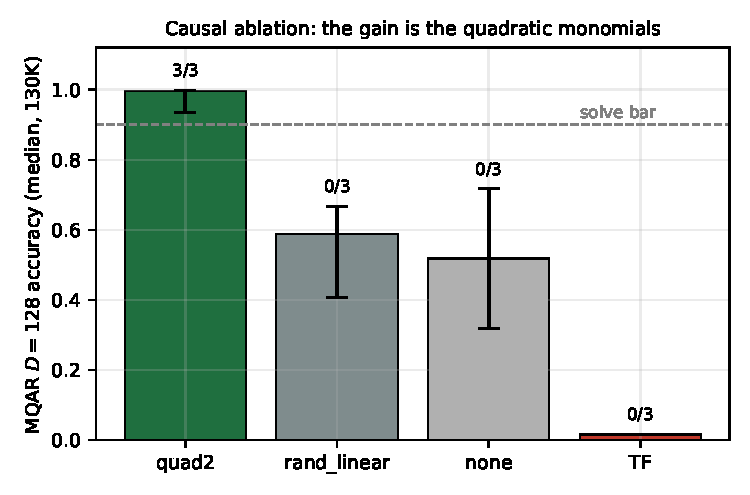
\includegraphics[width=0.62\linewidth]{fig5_ablation.pdf}
\caption{Causal control at 130K (d64L2H2, MQAR $D{=}128$, 3 seeds; error bars span the seed range).
Only \quadtwo{} clears the bar (3/3); \texttt{rand\_linear} (a $\dphi{=}256$ random \emph{linear}
lift) behaves like no feature map, and both sit far below \quadtwo. The recall gain is the quadratic
monomials, not state width. Data: \texttt{results/gpu\_bench.json}.}
\label{fig:ablation}
\end{figure}

The \texttt{rand\_linear} control is a same-dimension random \emph{linear} map (rank $\leq\dhd$, so it
expands $\dphi$ to 256 without adding any nonlinear structure). It performs like the no-map baseline,
not like \quadtwo. This isolates the effect: the recall gain comes from the \emph{quadratic monomials}
specifically, not from any $\dphi{=}256$ widening of the state. Only \quadtwo{} solves $D{=}128$ at
130K parameters.

\section{Limitations}
\label{sec:limits}

We state every limit plainly; the project's credibility rests on not inflating the claim.
\begin{enumerate}
\item \textbf{Char-LM is within-margin, not a win.} On text8 Prizma-Seq is competitive
\emph{within} the pre-registered $+0.05$ bar (1.7496 vs.\ 1.7254 BPC) but does \textbf{not} beat the
Transformer.
\item \textbf{Training is $\sim$5$\times$ slower per step.} The sequential delta recurrence makes
Prizma-Seq $\sim$5$\times$ slower to train (char-LM: 1889\,s vs.\ 361\,s per arm).
\item \textbf{Latency win is long-context-only.} The measured per-step latency crossover is at
$n{\geq}32$k; below $\sim$16k Prizma-Seq is $\sim$1.3--1.6$\times$ slower. The memory advantage holds
at all lengths; the latency advantage does not.
\item \textbf{No per-FLOP claim.} Prizma-Seq costs $2.14\times$ (as-coded; $1.78\times$
kernel-ideal) the Transformer's forward FLOPs per token at the headline scale. The two FLOP-matched Transformer arms (d128L9H4: 1/3; d208L4H4: 0/3,
median 0.022) were optimization-confounded (consistent with a learning-rate-transfer artifact, since
the same-depth narrower d128L4H4 solves), so they are excluded from the verdict and we make
\textbf{no per-FLOP claim}. Equal-parameter parity already addresses ``is it just compute?''.
\item \textbf{Seeds are descriptive, not powered.} $n{=}3$ (diagnostics) / $n{=}2$ (char-LM) support
failure-to-reject / descriptive parity, not a powered equivalence test. The diagnostic legs ran at a
single shared $\text{lr}{=}10^{-3}$ (conservative for Prizma-Seq) and their per-seed init is not
bit-pinned by the seed.
\item \textbf{Length-extrapolation is relative.} Prizma-Seq retains $10\times$ more accuracy than a
RoPE Transformer at $8\times$ train length, but its own absolute accuracy at $8\times$ is only
$\sim$0.40.
\item \textbf{No large-scale-LM parity and no backprop-free parity claim.} We test $\leq$3.2M
parameters at character level; large-scale LM parity and backprop-free parity are open frontiers,
explicitly not claimed.
\item \textbf{The kernel is borrowed.} \quadtwo{} belongs to the Based/Hedgehog feature-map family;
the novelty is the \emph{rectangular delta-state framing}, not the kernel.
\end{enumerate}

\section{Related work}
\label{sec:related}

\textbf{Linear and feature-map attention.} Linear attention~\cite{katharopoulos2020transformers,
choromanski2021performer} reframes attention as a recurrence with a fixed-size state. Based and
Hedgehog~\cite{arora2024based,zhang2024hedgehog} restore the recall lost by linearization through
expressive feature maps, including quadratic ones; we credit the \quadtwo{} kernel to this family.
Our contribution relative to them is the \emph{rectangular} ($\dhd\times\dphi$) delta-state framing
and its parameter-free, fixed-seeded-buffer instantiation.

\textbf{Delta-rule and gated recurrences.} The delta rule connects to fast-weight
programmers~\cite{schlag2021linear}; DeltaNet~\cite{yang2024deltanet} parallelizes it over sequence
length, and Gated DeltaNet~\cite{yang2024gateddeltanet} adds a data-dependent gate, as in
Mamba~\cite{gu2024mamba}. Prizma-Seq's mixer at the parallelizable level coincides with Gated-DeltaNet
plus a short conv and a local window head --- all borrowed, known-good components; we make this
explicit rather than presenting a new primitive.

\textbf{State-space models.} S4~\cite{gu2022s4}, Mamba~\cite{gu2024mamba}, and the SSM-attention
duality~\cite{dao2024mamba2} establish constant-state sequence mixing; Griffin~\cite{de2024griffin}
combines gated recurrences with local attention, motivating our window head.

\textbf{Recall diagnostics.} MQAR and the Zoology suite~\cite{arora2024zoology} are the
field-standard probes for the recall--efficiency tradeoff; our pre-registered bar uses them
directly.

\textbf{Predictive coding.} The free-energy reading of the delta write
draws on predictive coding~\cite{rao1999predictive,friston2010free}; the optional local/random-feedback
training mode relates to direct feedback alignment~\cite{nokland2016dfa} and is a secondary axis, not
a gate here.

\section{Conclusion}
\label{sec:conclusion}

Prizma-Seq is a Gated-DeltaNet--family sequence mixer whose only lever is a parameter-free quadratic
feature map (\quadtwo) that makes the carried delta-state rectangular ($\dhd\times\dphi$) at zero
added parameters and with $O(1)$ inference preserved. Parameter-matched against a tuned Transformer
it clears a pre-registered diagnostic bar at small scale: descriptive MQAR parity at 860K params,
$\geq$3.5$\times$ parameter-efficiency at 130K, solved induction and selective-copy, a within-margin
character LM, constant-memory inference with a long-context latency crossover, and a causal ablation
attributing the gain to the quadratic monomials. It is a \emph{candidate} efficient-attention
replacement in the tested regime --- not a proven alternative. The open frontiers we do not claim
are large-scale LM parity, per-FLOP advantage, and backprop-free parity.

\bibliographystyle{plain}
\bibliography{refs}

\end{document}
